%\title{Project Report}
%
%%% Preamble
\documentclass[paper=a4, fontsize=11pt]{scrartcl}
\usepackage[T1]{fontenc}
\usepackage{fourier}
\usepackage{listings}

\usepackage[english]{babel}															% English language/hyphenation
\usepackage[protrusion=true,expansion=true]{microtype}	
\usepackage{amsmath,amsfonts,amsthm} % Math packages
\usepackage[pdftex]{graphicx}	
\usepackage{url}
\usepackage{hyperref}
\usepackage{graphicx}
\usepackage{wrapfig}
\usepackage[margin=0.75in]{geometry}

%%% Custom sectioning
\usepackage{sectsty}
\allsectionsfont{\centering \normalfont\scshape}


%%% Custom headers/footers (fancyhdr package)
\usepackage{fancyhdr}
\pagestyle{fancyplain}
\fancyhead{}											% No page header
\fancyfoot[L]{}											% Empty 
\fancyfoot[C]{}											% Empty
\fancyfoot[R]{\thepage}									% Pagenumbering
\renewcommand{\headrulewidth}{0pt}			% Remove header underlines
\renewcommand{\footrulewidth}{0pt}				% Remove footer underlines
\setlength{\headheight}{3.6pt}
\date{}


%%% Equation and float numbering
\numberwithin{equation}{section}		% Equationnumbering: section.eq#
\numberwithin{figure}{section}			% Figurenumbering: section.fig#
\numberwithin{table}{section}				% Tablenumbering: section.tab#


%%% Maketitle metadata
\newcommand{\horrule}[1]{\rule{\linewidth}{#1}} 	% Horizontal rule

\title{
		\vspace{-1in} 	
		\usefont{OT1}{bch}{b}{n}
		\normalfont \normalsize \textsc{Durham Computer Science} \\ [5pt]
		\horrule{0.5pt} \\[0.4cm]
		\huge  GPU, Many-core and Cluster Computing Assignment - LLLL76\\
		\horrule{2pt} \\[0.5cm]
		\vspace{-1in} 	
}

%%% Begin document
\begin{document}
\maketitle
\section{Step One}
Report demonstrates a mastery of performance analysis tools (5). Bottleneck of codes are identified and characterised (5). Performance model is set up in the report and it is calibrated to the used machine and code (5). Some reasonable predictions are made how much can be improved by performance optimisation (5).
\subsection{Results}
\begin{figure}[h]
\caption{}
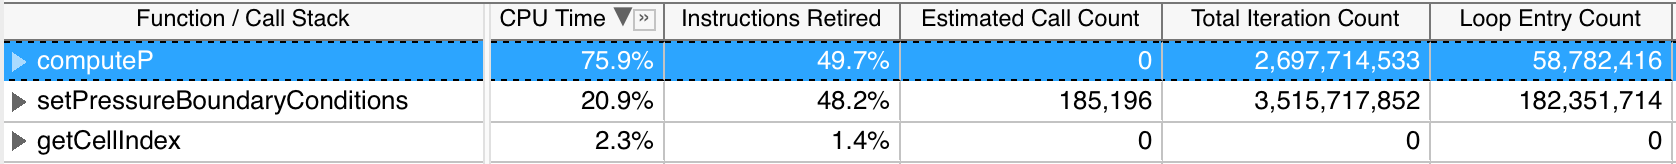
\includegraphics[width=\textwidth]{one.png}
\end{figure}
\begin{figure}[h]
\caption{}
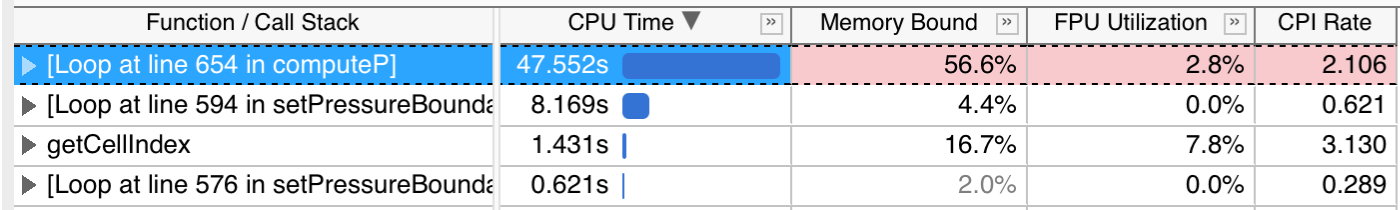
\includegraphics[width=\textwidth]{two.png}
\end{figure}

This run time analysis is taken from Vtune. It was used on a slightly altered step one, all IO has been turned off as to give an accurate representation of the computational time of the program and not the IO. This was also run on Hamilton so the processes do not share CPU cycles or RAM.

- Talk about compiler optimisation variants
- All IO is removed so as to remove superfluous stuff
- Used hamilton to run so as to get pure results
- would a different machine make a difference
- model would probably be amdals
- this program will be memory bound
- differences that parameters make

\subsection{Bottlenecks}

The bottle neck, as shown above is the loop in the function 'computeP'. This takes up a very large amount of the CPU Time. Another computationally significant part of the code is the function 'setPressureBoundaryConditions', whilst this does not make up as much of the CPU time as 'computeP' it is still a significant percentage.

\subsection{Performance Model}

\subsection{Predictions}

%%%%%%%%%%%%%%%%%%%%%%%%%%%%%%%%%%%%%%

\section{Step Two}
Report gives a clear description what has been realised in the code (5). Vectorisation report results are summarised in report and discussed (5). Runs with various input data sets have been made (5). Results are presented with state-of-the-art techniques (proper figures, e.g.) (5).
\subsection{Description}

In step two we work to split the computational domain into smaller cubes and vectorise any parts that can be.  A loop can be vectorised if it meets a certain criteria; it must be countable, meaning that the number of iterations must be known before we enter the loop, it must have only a single entry and a  single exit, it also must have no branching, ie no if statements. The other criteria is only inner loops, no function calls, and no internal dependencies. 

The criteria that this code breaks is the fact that it's main loop in the 'computeP' function contains branching, if this was removed then this loop could be vectorised as it meets all other criteria. We start by splitting the overall box we are working in into smaller cubes, the dimensions of these cubes is hard-coded at a single point in the code, this is easy to change. If the dimensions of the box is such that it cannot be made up of complete cubes then the code will halt. If the input variables are such that the box can be made up of a whole number of cubes then the code will move onto working out if a given cube can be vectorised, this would be the case if, out of all the cells in the given cube, none of them are part of the obstacle. If the given block contains no cells from the obstacle then it can be vectorised as in the standard realisation of the code the if statement is a check if the current cell is part of the obstacle. Thus the pre-processing for checking the status of the cells is required to allow the non-obstacle blocks to be vectorised and the blocks that do contain part of obstacle to be treated with the standard code given, using the if statement.

The stages of the vectorisation are as follows, pre-processing takes place, this will check all cells in each block and set a flag as to what is contained within the block, obstacle or not. This will then be used to choose which set of for loops should be used, the vectorised or non-vectorised. The vectorisation is done using the standard intel SIMD pragma.

The pragma SIMD alters the order of cell propagation, the order is now block by block rather than cell by cell the overall effect is negligible.

\subsection{Vectorisation Reports}

The vectorisation report for the unvectorised version of the code shows that the function "ComputeP" has no vectorised parts.
\begin{lstlisting}

LOOP BEGIN at gpu1.cpp(659,9)
        remark #15344: loop was not vectorized: vector dependence prevents 
        vectorization. First dependence is shown below. Use level 5 report for details
        remark #15346: vector dependence: assumed ANTI dependence 
        between _rhs[_ix+_iy*(_numberOfCellsPerAxisX+2)+(_iz*(_numberOfCellsPerA (670:25) 
        and _p[$i4] (673:13)
LOOP END

\end{lstlisting}

There are two loops that are present in step two, one that is vectorised and allowed for blocks that do not contain any parts of the obstacle to avoid the if statement in the standard loop that is unvectorised. 

\begin{lstlisting}

 LOOP BEGIN at gpu21.cpp(594,17)
		remark #15301: SIMD LOOP WAS VECTORIZED
 LOOP END

\end{lstlisting}

This is the vectorised loops vec-report, the other loop is almost identical to the loop in step one.

\subsection{Results}

TO BE DONE AT HOME

%%%%%%%%%%%%%%%%%%%%%%%%%%%%%%%%%%%%%%

\section{Step Three}
Report gives a clear description what has been realised in the code (5). Runs with various input data sets have been made (5). Results are interpreted and future work and shortcomings are identified (5). Results are presented with state-of-the-art techniques (proper figures, e.g.) (5).
\subsection{Description}

- The arrays that store all values for the cells are padded in such a way that there is a layer of cells surrounding each block.\\
- at the beginning of each computeP iteration the values of the padded cells are changed to the values of their corresponding non padded cell. (Give a visual example of this)\\
- This is done via a conversion function that will take in the index of the halo cell and will return the correct value of that halo.\\
- all other functions that contain loops that used to iterate through the standard array are unchanged however the function call has been changed such that the values passed for the original array are mapped to the corresponding cell in the padded array, this is easier as a mapping function being called instead of changing all for loops in the program is more simple.\\
- the only place that a padded array can be used is inside the function computeP, in any other function this array cannot be accessed, and thus we write out to the unpadded array after each iteration.\\
- each padded block is then passed through the OMP parallel pragma such that it is done in parallel using the padded values for any data that would otherwise be from a different block and would thus not allow for parallel as it would introduce data races. After this has been then we will go into a different iteration which would result in the new halo values being written from their corresponding non halo cell.. 

\subsection{Results}

\subsection{Limitations}

- overhead
- inaccuracy?
- a lot of copying data

%%% End document
\end{document}